\chapter{Preliminaries}\label{chapter:preliminaries}

\section{Space Plasma}\label{sec:plasma}

Plasma is ubiquitous throughout the visible Universe, also known as the fourth state of matter 
due to its properties which differentiate it from the conventional gaseous state. Plasma is a 
gas which is composed of roughly equal number of positive and negatively charged particles, this
property is known as charge \emph{quasi-neutrality}. The term quasi-neutral is used because although
the gas has almost equal amount of positive and negative charges, the mixture is electricomagnetically 
active. Due to incomplete charge sheilding, long range electromagnetic fields play a big role in the 
dynamics of plasma.

From classical electrostatics the electric potential of a point charge $q$, is given as

\begin{equation}
    \phi(r) = \frac{q}{4\pi\epsilon_0 ||r||_2}
\end{equation}

where $r$ is the position in space with respect to the charge and $\epsilon_0$ is the \emph{permitivity} of vacuum.

\subsection*{Debye Length}

In a quasi-neutral plasma, due to the prescence of partial electric sheilding the potential due to the charge 
now takes the so called Debye form.

\begin{equation}
    phi(r) = \frac{q}{4\pi\epsilon_0 ||r||_2} e^{-\frac{||r||_2}{\lambda_d}}
\end{equation}

The electric potential decays with the Debye length scale $\lambda_d$ at which a balance between thermal vibrations 
which can disturb quasi-neutrality and electrostatic forces due to charge separation. The Debye length scale depends
on the electron temperature and plasma density.

\begin{equation}\label{eq:debye}
    \lambda_d = \sqrt{\frac{\epsilon_0 k_b T_e}{n_e e^2}}
\end{equation}

In equation \ref{eq:debye}, the Debye length scale is expressed in terms of the \emph{Boltzmann constant} $k_b$, 
the electron temperature $T_e$, free space permitivity $\epsilon_0$ and electron charge $e$. One can visualise the 
positively charged ions having a cloud of electrons sheilding them at the distance of $\lambda_d$. 

It is also possible to take into account the sheilding effect of the ions. The effective Debye length is now 
expressed as an addition of two terms, one for electrons (\ref{eq:debye}) and a similar term for the ions by replacing 
$T_e$ for the ion temperature $T_i$ ($n_i \approx n_e$). 

\subsection*{Plasma Parameter}

Consider a Debye sphere of radius $\lambda_d$, this sphere contains $N_e = \frac{4}{3}\pi \lambda^3_d n_e$ electrons. The 
plasma parameter $g$ is defined as $N_{e}^{-1}$. Rewriting this, we can say:

\begin{equation}
    g \sim \sqrt{\frac{n_e}{T_e}}
\end{equation}

The description of plasma used in many applications in Space is applicable when $g \|| 1$, in this situation the Debye sheilding 
is significant and the quasi-neutral plasma obeys collective statistical behaviour. The plasma parameter $g$ also correlates with 
the collision frequency. As the collisions in plasma increase with increasing density and decreasing temperature, if $g \longrightarrow 0$ 
the plasma becomes nearly collisionless. The collisionless property helps in making simplfying assumtions about plasma dynamics and 
is the starting point for the \emph{adiabatic} theory of plasma motions in the Earth's magnetosphere which will be discussed in section 
\ref{sec:plasmadiff}.

\section{Sun \& the Solar Wind}\label{sec:solar}


\begin{figure}
    \noindent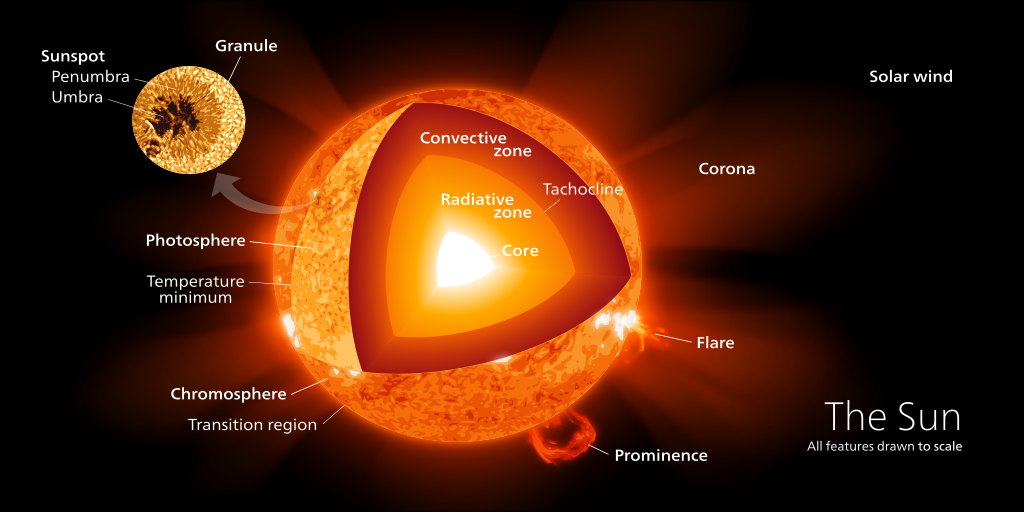
\includegraphics[width=\textwidth]{Sun_poster.png}
    \caption{\small Cross section of the Sun \\ Author: Kelvinsong [CC BY-SA 3.0 (\url{https://creativecommons.org/licenses/by-sa/3.0})] \\ Source: Wikipedia}
    \label{fig:SunLayers}
\end{figure}

%\begin{wrapfigure}{r}{0.4\textwidth}
%    \centering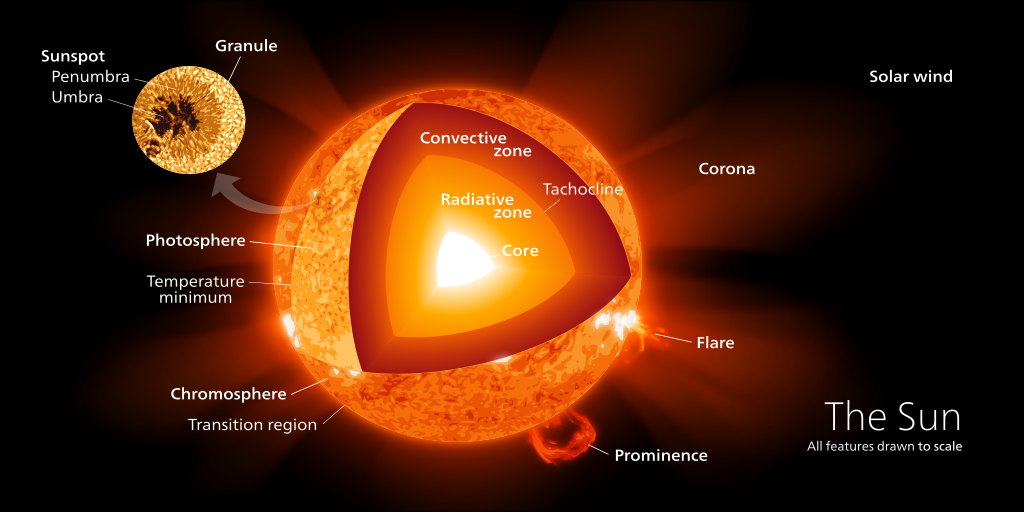
\includegraphics[width=0.38\textwidth]{Sun_poster.png}
%    \caption{
%        \small Cross section of the Sun \\ Author: Kelvinsong [CC BY-SA 3.0 (\url{https://creativecommons.org/licenses/by-sa/3.0})] \\ Source: Wikipedia}
%    \label{fig:SunLayers2}
%\end{wrapfigure}



\section{Magnetosphere}\label{sec:mag}

\subsection*{Particle Motions \& Adiabatic Theory} \label{sec:plasmadiff}

